\chapter{Programación de Placas Gráficas}

\section{Introducci\'on}
La constante demanda de poder en las aplicaciones gr\'aficas, motivada sobre todo por el auge de los videojuegos y las películas de animación, han provocado que el poder de cómputo de las unidades de hardware paralelo haya sufrido una marcada evoluci\'on desde su aparici\'on.
Dicha evoluci\'on ha tenido como consecuencia la rivalizaci\'on y posterior superaci\'on por parte de las GPU's al poder de procesamiento con el que cuentan las CPU's tradicionales\cite{Harris06}.
En la siguiente sección se comenta la historia de la programación de las placas gráficas.

\section{Historia del Shader Programable}
Las placas gráficas o GPUs son microprocesadores, y por lo tanto tienen su propio lenguaje assembler, el cual puede programarse para realizar una tarea específica.
A diferencia de las CPUs, las GPUs no son herramientas de propósito general, sino que son microprocesadores adaptados a realizar tareas gráficas, como manejar triángulos, líneas y puntos.
Estos microprocesadores han ido evolucionando a lo largo de los años, donde distintas compañías han hecho su aparición.
Debido a esto, existen (al igual que ocurre con las CPUs) distintos lenguajes assembler, y distintas arquitecturas de GPUs.
Por lo cual, cada placa debe programarse bajo su propio lenguaje.
El diseño orientado a elementos repetitivos e independientes como píxels, triángulos y vértices en los que se descompone una escena en computación gráfica ha resultado en un diseño {\em paralelo} de las mismas.
Actualmente, las placas gráficas cuentan con miles de procesadores (aunque más limitados que un microprocesador CPU), los cuales realizan tareas como actualizar un píxel, o establecer la proyección perspectiva de un vértice en pantalla.
Este procesamiento se hace en paralelo ya que la computación es independiente para cada elemento.

En un principio, la placa gráfica funcionaba como una caja gris o negra, la cual podía ser configurada únicamente, para producir resultados limitados sobre algunos tipos de efectos, como el color final de un píxel.
En la década de $1980$ comenzaron a surgir las placas gráficas programables, donde era posible modificar el assembler de determinados procesos de las mismas, logrando efectos personalizados.
El assembler de estas placas no resultaba nada amigable al progrmador, además de ser distinto para cada placa, por lo cual un programador debía distribuir código assembler para cada placa donde pretendía correr su programa.

De igual forma que ocurrió con la aparición de los lenguajes de programación de propósito general como C, COBOL o Lisp, comenzaron a surgir, aproximadamente en el año $2000$ lenguajes más amigables para el programador que compilaban al assembler específico de cada GPU.
De esta forma surgieron GLSL\footnote{OpenGL Shading Language} (OpenGL, por lo tanto, libre), HLSL (Microsoft) y Cg (nVidia).
De ellos, el primero es el único que compila para diferentes plataformas, ya que los otros dos están orientados a dispositivos de sus respectivas empresas (por ejemplo, Cg no se puede utilizar en placas ATI).

Los lenguajes de shading probaron ser una herramienta flexible y poderosa para controlar el comportamiento y apariencia de objetos en una escena.
Se han codificado algoritmos de iluminación, sombreado, de generación de vértices, superficies y un largo etc. en shaders, lo cual significó un gran trasvasamiento de cómputos del CPU al GPU.

A medida que las placas se hicieron más poderosas, resultó evidente la posibilidad de utilizar las mismas como unidad de propósito general.
El modelo de computaci\'on paralelo con el que cuentan las mismas, hizo surgir herramientas que permiten derivar todo el c\'alculo hacia el hardware secundario, conoci\'endose este modelo de computaci\'on como {\em GPGPU}\footnote{General-Purpose Computing on Graphics Processing Units}.
El cómputo GPGPU cuenta a grandes rasgos con la siguiente secuencia de pasos: copia de memoria y datos desde el CPU al GPU, cómputo en el GPU, y paso de los resultados desde el GPU al CPU (posiblemente modificando datos y memoria).
Es decir, la GPU sólo estaría {\em prestando} su funcionamiento al CPU, para un propósito para el que no fue hecho, el cual es realizar cómputos generales en paralelo.
Debido a que los CPUs encontraron un límite físico en cuando a la velocidad que podían alcanzar (unos cuantos gigahertz o GHz), la aparición de las CPUs permitió, en el ámbito hogareño y empresarial (entre otros) seguir aumentando los TeraFlops\footnote{Unidad de medida, 1 TeraFlop = $10^{12}$ intrucciones de coma flotante por segundo.}, de manera similar a la utilización de un cluster o de microprocesadores de varios núcleos, aunque estos últimos nunca pudieron alcanzar la velocidad de las GPUs modernas.

El principal problema de esto es la copia de memoria desde y hacia la placa, lo cual puede resultar muy costoso.
Debido a esto, en los últimos años se han desarrollado modelos de memoria unificada, donde la CPU y la GPU compartirán la memoria.


% las placas gr\'aficas acabar\'an por reemplazar a los CPU's existentes hoy en d\'ia. A continuaci\'on se presentan dos ejemplos de las tecnolog\'ias mencionadas.
% En primer lugar se discute el lenguaje de shading utilizado en el framework. En segundo lugar se muestra un ejemplo de una biblioteca de GPGPU muy conocida hoy en d\'ia, la cual fue utilizada para el c\'alculo de texturas offline.

\section{El lenguaje GLSL}
%La palabra Cg significa ``C para gr\'aficos'', en alusi\'on al bien conocido lenguaje de programaci\'on C. Esto implica que Cg es un lenguaje tambi\'en, siendo su principal novedad que el mismo est\'a dise\~nado para producir c\'odigo {\em Assembler} de la placa gr\'afica de la computadora (GPU). El mismo nos permite controlar la apariencia, movimiento y forma de los objetos dibujados usando la GPU \cite{Randima03}. Cg no es un lenguaje de prop\'osito general, sino que est\'a completamente orientado a trabajar sobre elementos gr\'aficos como v\'ertices, p\'ixeles, l\'ineas, pol\'igonos, vectores, etc.; su nombre est\'a basado en C s\'olo por su sintaxis, lo cual le otorga un parecido al mismo. Este tipo particular de lenguajes reciben el nombre de {\em Shading languages} (lenguajes de Shading), aunque como se ver\'a m\'as adelante, el lenguaje permite realizar otras clases de operaciones.

La principal ventaja de usar la GPU consiste en la {\em velocidad}. La CPU ({\em Central Processing Unit}) delega las operaciones gr\'aficas hacia el hardware gr\'afico programable, el cual realizar\'a el procesamiento en un marco especializado, quedando as\'i liberado el primero para realizar tareas m\'as acordes con el procesamiento general de los programas
Esto implica entonces una tarea conjunta entre CPU y GPU.


\subsection{El pipeline Gr\'afico y GLSL}
As\'i como en la CPU, la GPU posee un {\em pipeline}, esto es, una secuencia ordenada de pasos por cada instrucci\'on de procesamiento.
En primer lugar, es la CPU quién se comunica con la GPU para enviarle la información gráfica a ser procesada, esto consiste generalmente de una escena descompuesta en triángulos, pero además existen otros datos como las texturas a ser aplicadas, los cuales también son provistos.
En la GPU, de manera análoga a la CPU, se cuenta con una unidad de procesamiento y una unidad de memoria.
A diferencia del CPU, la arquitectura de la misma presenta una memoria estratificada, y un diseño paralelo de la unidad de procesamiento.

Cada procesador cuenta con una memoria propia (local).
Los procesadores se organizan en grupos, los cuales contienen una memoria para el grupo.
Finalmente, existe una memoria global, la cual permite la comunicación entre todos los procesadores.
Los accesos a las distintas memorias tienen distintos costos.
La memoria global es la más costosa, computacionalmente, siendo la memoria propia de cada procesador la más rápida.

La GPU recibe los datos desde la CPU y comienza su procesamiento.
Luego del procesamiento, los resultados son volcados en una memoria especial del GPU, denominada {\em framebuffer}, el cual es el puente entre la placa de video y el monitor.
Este es el escenario típico, excepto en los casos de GPGPU, donde la placa se utiliza para otros propósitos, y por lo tanto los resultados no son imágenes.
Una vez que se cuenta con los vértices, líneas, triángulos, texturas, etc. a ser renderizados, debe transformarse la información tridimensional en información bidimensional para ser representada en la pantalla del monitor.
La secuencia t\'ipica de procesamiento de la GPU est\'a ordenada de la siguiente manera:
\begin{itemize}
\item Procesamiento de V\'ertices: los v\'ertices de los objetos de una escena llegan desde el programa. Este es el primer momento en el que interviene GLSL. Se da lugar entonces a la transformaci\'on personalizada por el programador sobre los mismos. Este tipo de transformaciones son las usuales sobre los v\'ertices: rotaci\'on, desplazamiento, etc.
\item Ensamblamiento y Conversi\'on Scan: aqu\'i estos v\'ertices transformados son unidos para formar l\'ineas, puntos y tri\'angulos, mediante la informaci\'on que llega desde el programa junto con los v\'ertices. Luego, se realizan los procesos de {\em clipping}: eliminaci\'on de partes de objetos que por su posici\'on no aparecer\'an en pantalla; y {\em culling}: eliminaci\'on de superficies no visibles, puesto que est\'an detr\'as de otras superficies desde el punto de vista de la c\'amara. Aquellas partes que pasan estos filtros, son luego {\em rasterizadas}, esto es, {\em asociadas} a posiciones en pantalla; puntos, l\'ineas y tri\'angulos pasan entonces a tener una posici\'on determinada, este proceso se conoce como {\em conversi\'on scan}. Es as\'i que se generan los denominados {\em fragmentos}, los cuales pueden definirse como ``candidatos a ser p\'ixeles'': aquellos fragmentos que pasen filtros posteriores se convertir\'an en p\'ixeles que ser\'an representados en pantalla. Puede haber numerosos fragmentos que compitan por ser un p\'ixel. Es en este momento que GLSL hace su segunda aparici\'on, el programador decide entonces c\'omo quiere generar los fragmentos.
\item Interpolaci\'on, aplicaci\'on de texturas y colores: en esta etapa, los fragmentos generados en la etapa previa son {\em interpolados} (por ejemplo el color de los mismos), y luego se le aplican operaciones matem\'aticas y de texturas.
\item Operaciones de Raster: en esta \'ultima etapa se llevan a cabo una serie de tests sobre cada fragmento. Si alguno falla, el fragmento es descartado, de lo contrario el color del fragmento actualizar\'a el color del p\'ixel correspondiente. Un fragmento podr\'ia no sobrevivir a esta etapa porque debido a su profundidad queda detr\'as de otro fragmento.
\end{itemize}

En la GPU existen dos componentes llamados {\em procesador de v\'ertices programable} y {\em procesador de fragmentos programable}, los cuales se encargan de correr los programas GLSL escritos por el programador, respectivamente llamados {\em Vertex Shader} y {\em Fragment Shader}.

\begin{figure}[h]
\begin{center}
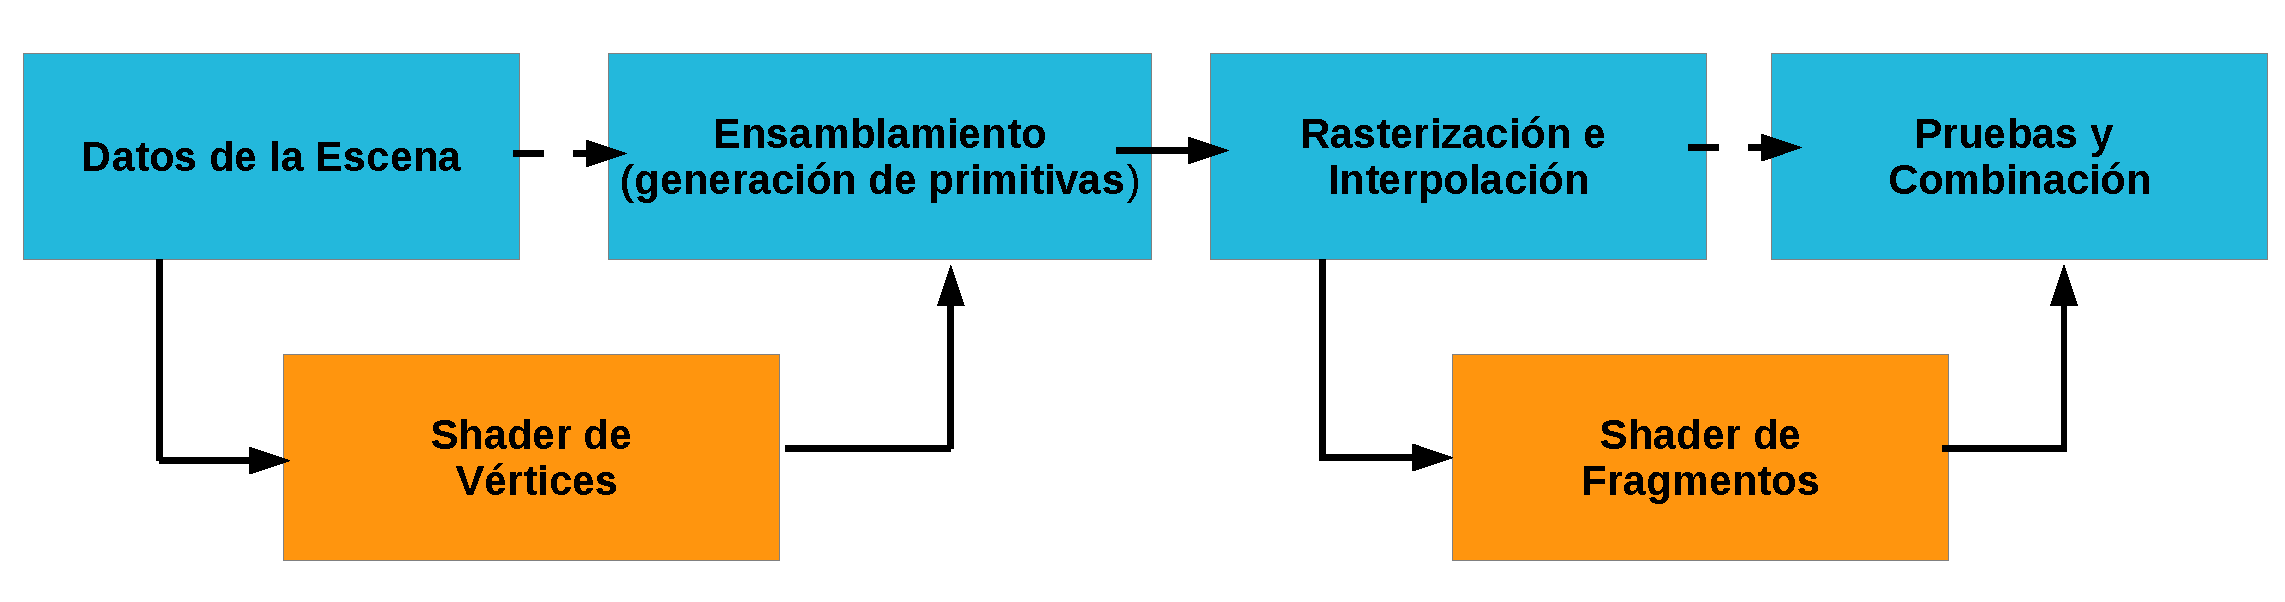
\includegraphics[width=13cm]{figures/pipelinegrafico}
\end{center}
\caption{Pipeline de la GPU con shaders incluídos.}
\label{fg:pipelinegrafico}
\end{figure}


\subsection{C\'omo usar GLSL en aplicaciones gr\'aficas}
%Cg ofrece una biblioteca conocida como su {\em runtime}. Bibliotecas como {\em OpenGL} o {\em Direct3D} deben comunicarse con el mismo para obtener los servicios que necesitan. Como componente del runtime, Cg posee un {\em compilador}, el cual traduce el c\'odigo Cg a alguno de los {\em Perfiles} existentes.
OpenGL incluye desde su versión $2.0$ una integración directa con el lenguaje, por lo que es posible programar los distintos shaders de manera transparente, es decir, sin necesidad de compilar o enlazar el código resultante, como sí ocurre en lenguajes rivales como Cg.

Como posible limitación, debe tenerse en cuenta la capacidad de la placa donde se correrá el programa.
Por ejemplo, determinadas placas no permiten bucles en el shader de fragmentos, o tienen un límite en el número de texturas que soportan, debido a limitaciones de hardware.
Para agrupar distintas tecnologías en un estándar, se definieron {\em perfiles}.

Un perfil es una combinaci\'on de las capacidades que otorgan la biblioteca y la GPU que poseemos para ejecutar los programas. Los perfiles en definitiva establecen limitaciones a lo que podemos lograr con un programa GLSL. Es as\'i que al compilar para un perfil determinado debemos tener en cuenta las restricciones del mismo. Sin embargo, la r\'apida evoluci\'on del hardware gr\'afico hace que las restricciones sean cada vez menores.

%Existen adem\'as dos bibliotecas que se encargan de tomar el programa traducido por el compilador Cg y pasarlo a la biblioteca gr\'afica que estamos utilizando: {\em cgGL} (OpenGL) y {\em cgD3D} (Direct3D). Este c\'odigo traducido es tomado por alguna biblioteca gr\'afica la cual luego se encargar\'a de que el mismo corra en la GPU.

%Antes de la aparici\'on de lenguajes como GLSL, el programador que pretend\'ia tener un cierto control sobre c\'omo renderizar una escena, deb\'ia programar directamente el assembler de la placa gr\'afica correspondiente. Esto supone una p\'erdida de generalidad, puesto que debe hacerse un programa distinto para cada placa que pretenda usarse, adem\'as de un conocimiento preciso sobre el juego de instrucciones y el funcionamiento de cada placa. Con Cg, el programador se abstrae de todo esto. 

\subsection{Caracter\'isticas de GLSL - Generalidades}
Presentamos un breve resumen de las pricipales caracter\'isticas del lenguaje.
Como fue previamente mencionado, existen dos tipos de programas en GLSL, siendo sus nombres {\em Shader de Vértices} y {\em Shader de Fragmentos} respectivamente.

La manera de definir qué se dibujará en pantalla dentro del pipeline de OpenGL 2.0+  es a través de atributos de vértices y elementos. 


Los \emph{atributos} son, como su nombre lo dice, atributos o propiedades de un vértice. El significado se los dará el uso, pero por lo general un atributo infaltable es la posición de cada vértice. Otros atributos comunes serán : normales, colores y coordenadas de texturas.
Los \emph{elementos} son figuras geométricas (lineas, triángulos, cuadrados) que se forman a partir de unir los vértices definidos por los atributos, ver Fig.~\ref{fg:atributos}.

\begin{figure}[h]
\begin{center}
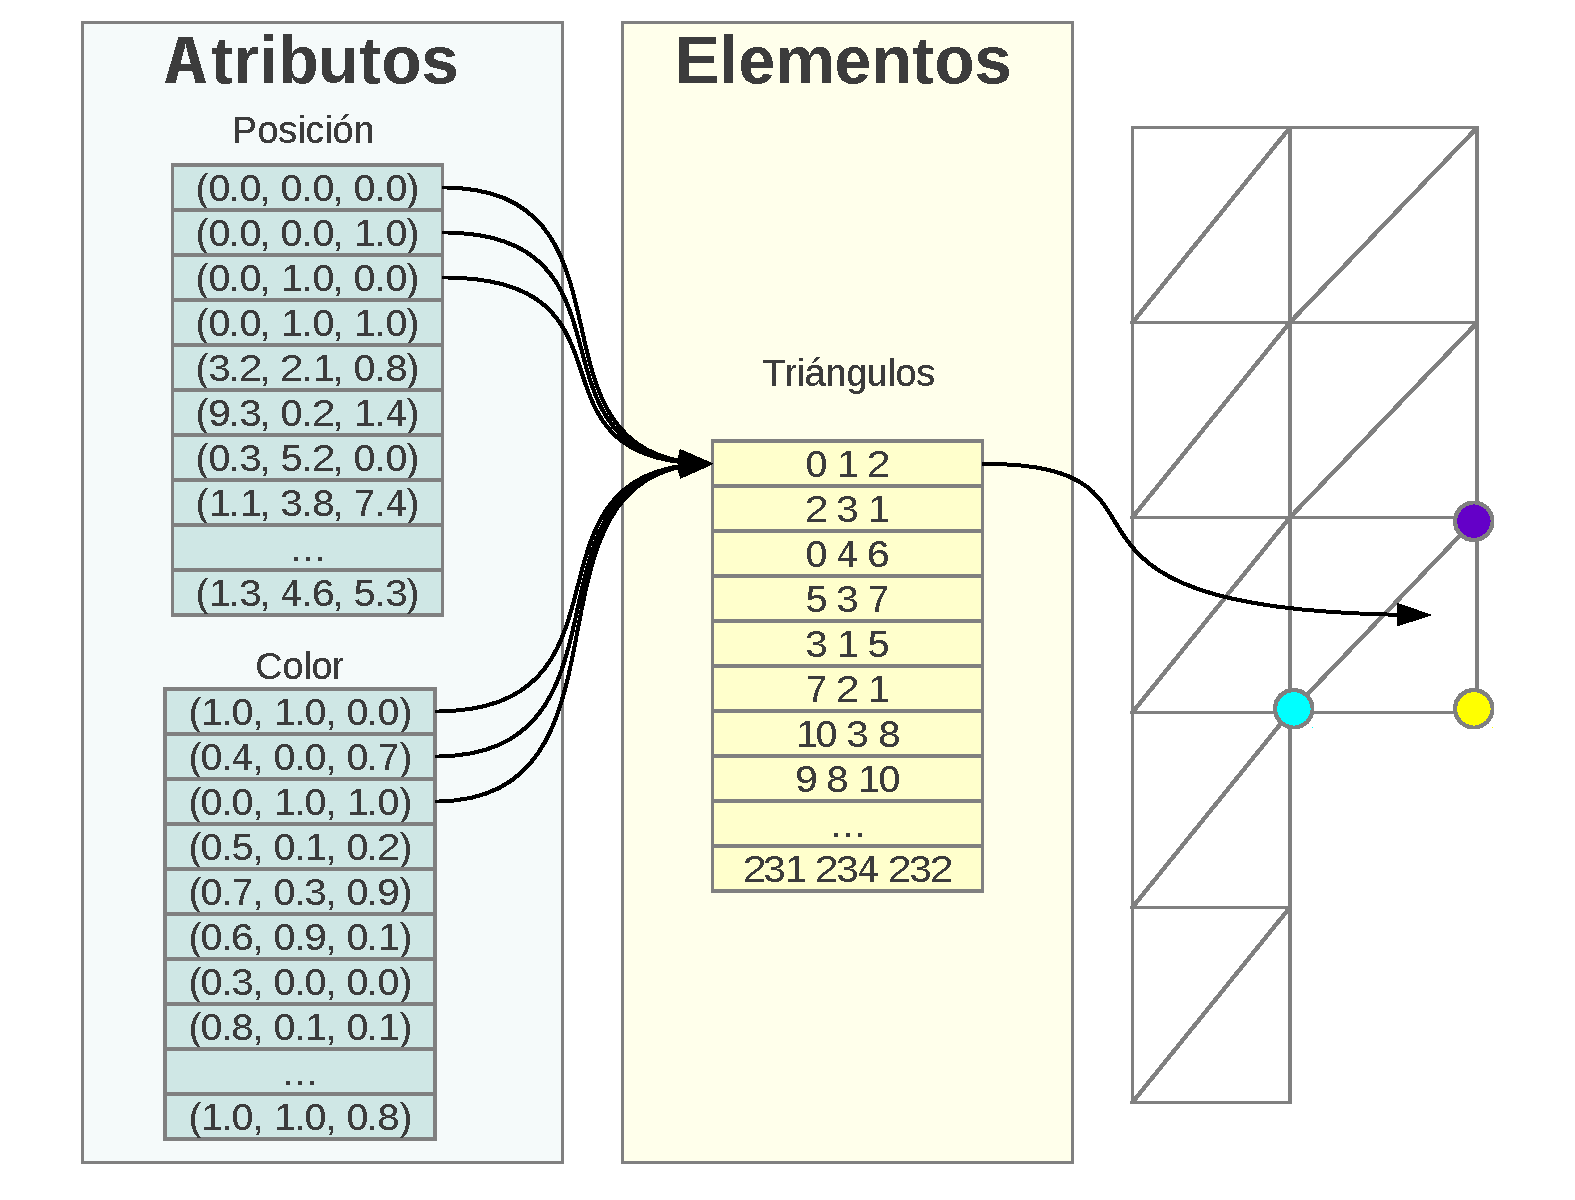
\includegraphics[width=13cm]{figures/atributos}
\end{center}
\caption{Atributos y elementos en GLSL.}
\label{fg:atributos}
\end{figure}

La funci\'on del shader de vértices es tomar los v\'ertices que llegan desde la aplicaci\'on gr\'afica, transformarlos y pasarlos al siguiente eslab\'on del pipeline.
De manera simplificada, este shader recibe como entrada la posici\'on del v\'ertice en la escena, y terminada la ejecuci\'on devolver\'a el v\'ertice con su posici\'on modificada.
Tambi\'en podr\'ia devolver el color y otros valores \'utiles que se puedan necesitar m\'as adelante.
Estos programas usan los atributos como entrada, asi como otras constantes llamadas \emph{uniformes} para definir la posición final en espacio de clipping de cada vértice.
Los valores \emph{uniformes} pueden ser por ejemplo las matrices de proyección y del modelo o matrices para transformar normales. 

La Fig.~\ref{fg:vertexshader} muestra un ejemplo de un shader de vértices junto a atributos de ejemplo.
El programa que puede observarse en la figura transforma el vértice de manera estándar utilizando las matriz de modelviewproj (modelo, vista, proyección), la cual es provista como un uniforme desde la CPU.
Los atributos intervinientes con el color y la posición del vértice.
La imagen muestra además que la variable gl\_Position es la salida del programa, la cual tiene coordenadas del espacio de clipping (entre $[-1,-1,-1]$ y $[1,1,1]$).

\begin{figure}[h]
\begin{center}
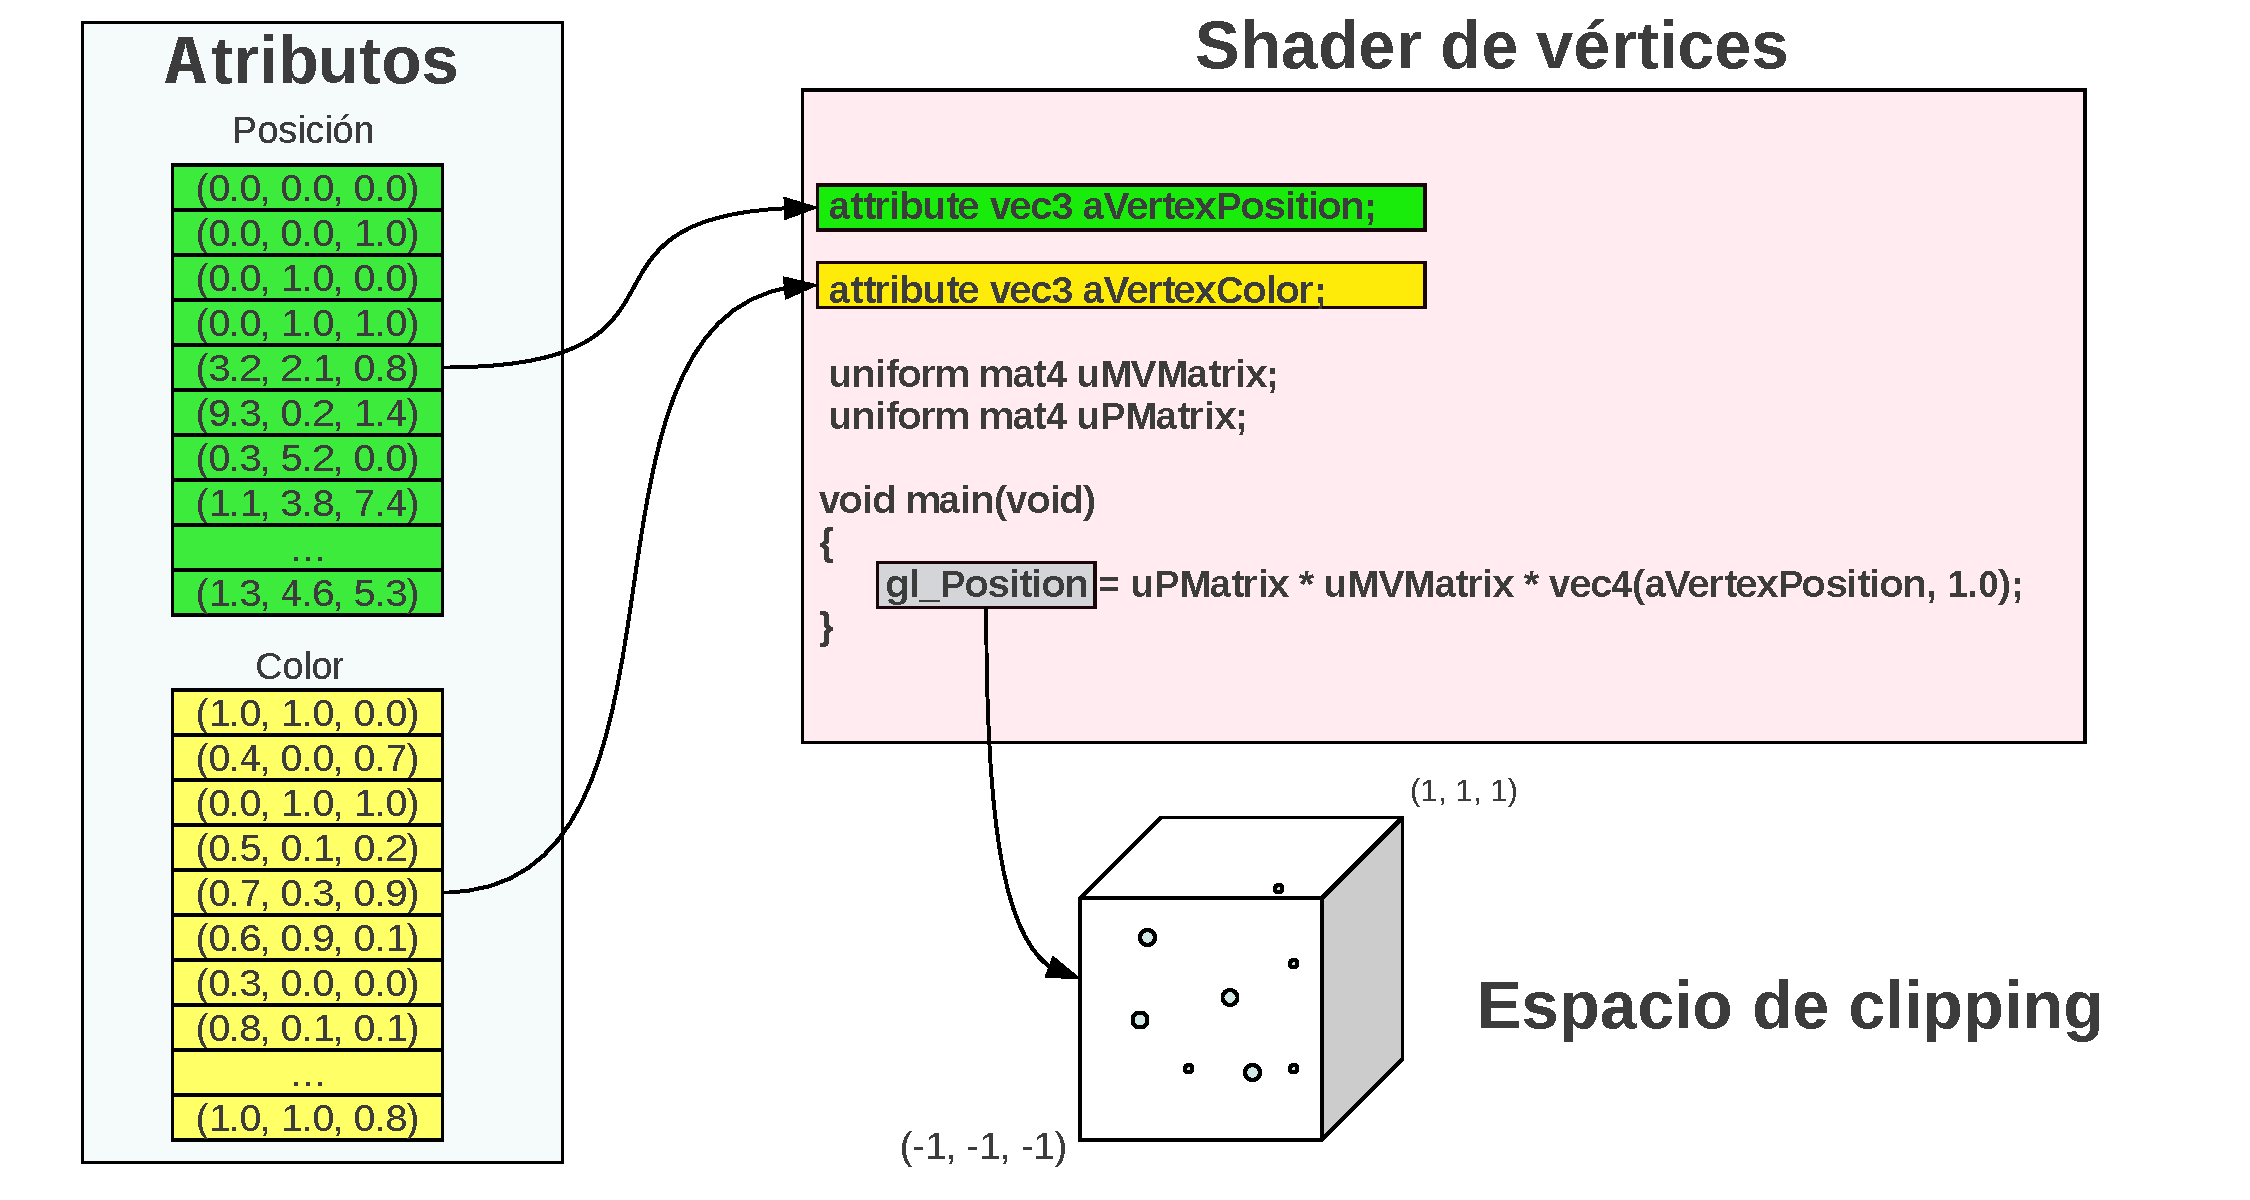
\includegraphics[width=13cm]{figures/vertexshader}
\end{center}
\caption{Atributos y elementos, junto a un ejemplo de shader de vértices en GLSL.}
\label{fg:vertexshader}
\end{figure}

Una vez que todos los shaders de vértices realizaron sus cómputos, debe procederse a la rasterización, es decir se calcula su posición final en la pantalla a partir de la información del tamaño de la imagen final requerida.
Cada elemento (triángulo, linea, cuadrado) se convierte en una grupo de pixeles (llamado fragmento) que posiblemente se pintará en la pantalla.
Este proceso puede observarse en la Fig.~\ref{fg:raster}, y a diferencia del vértice de fragmentos, no es programable.
Es decir, que está implementado en hardware por la placa gráfica y no es posible su modificación.


\begin{figure}[h]
\begin{center}
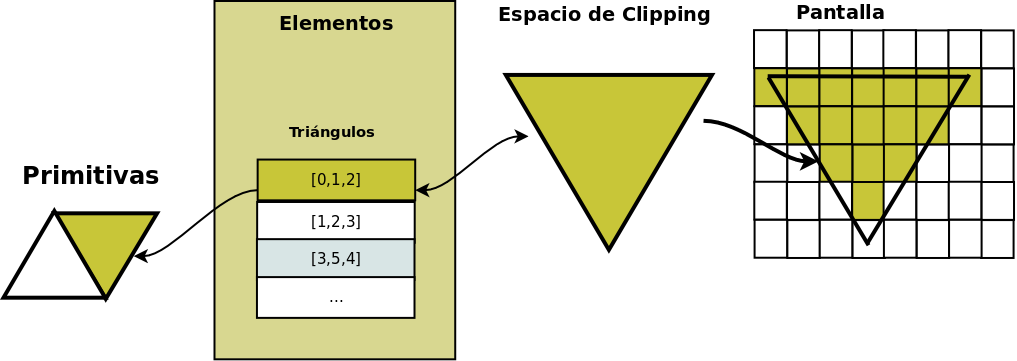
\includegraphics[width=13cm]{figures/raster}
\end{center}
\caption[Proceso de rasterización en la placa gráfica]{Proceso de rasterización en la placa gráfica. En la imagen, un triángulo es convertido al conjunto de las posiciones de los píxeles que representará en la pantalla.}
\label{fg:raster}
\end{figure}

Finalmente, para calcular el color de cada pixel en pantalla, se le pasa al pipeline un pequeño programa llamado \emph{shader de fragmentos} que calcula el color de cada pixel (o fragmento) que ocupa un elemento (triángulo, linea, cuadrado) individualmente.
Para computar el color final de cada píxel, se pueden pasar \emph{uniformes} al igual que a los \emph{shaders de vértices} y también se pueden pasar valores de un \emph{shader de vértices} a un \emph{shader de fragmentos}.
Los valores calculados para cada vértice se interpolan de acuerdo a la distancia al vértice del pixel cuyo color se está calculando.
Estos valores que pasan de un \emph{shader} a otro se declaran como \emph{varying} dentro de ambos.
La Fig.~\ref{fg:fragmentshader} muestra un ejemplo de la utilización de un varying para computar el valor interpolado de un triángulo.


\begin{figure}[h]
\begin{center}
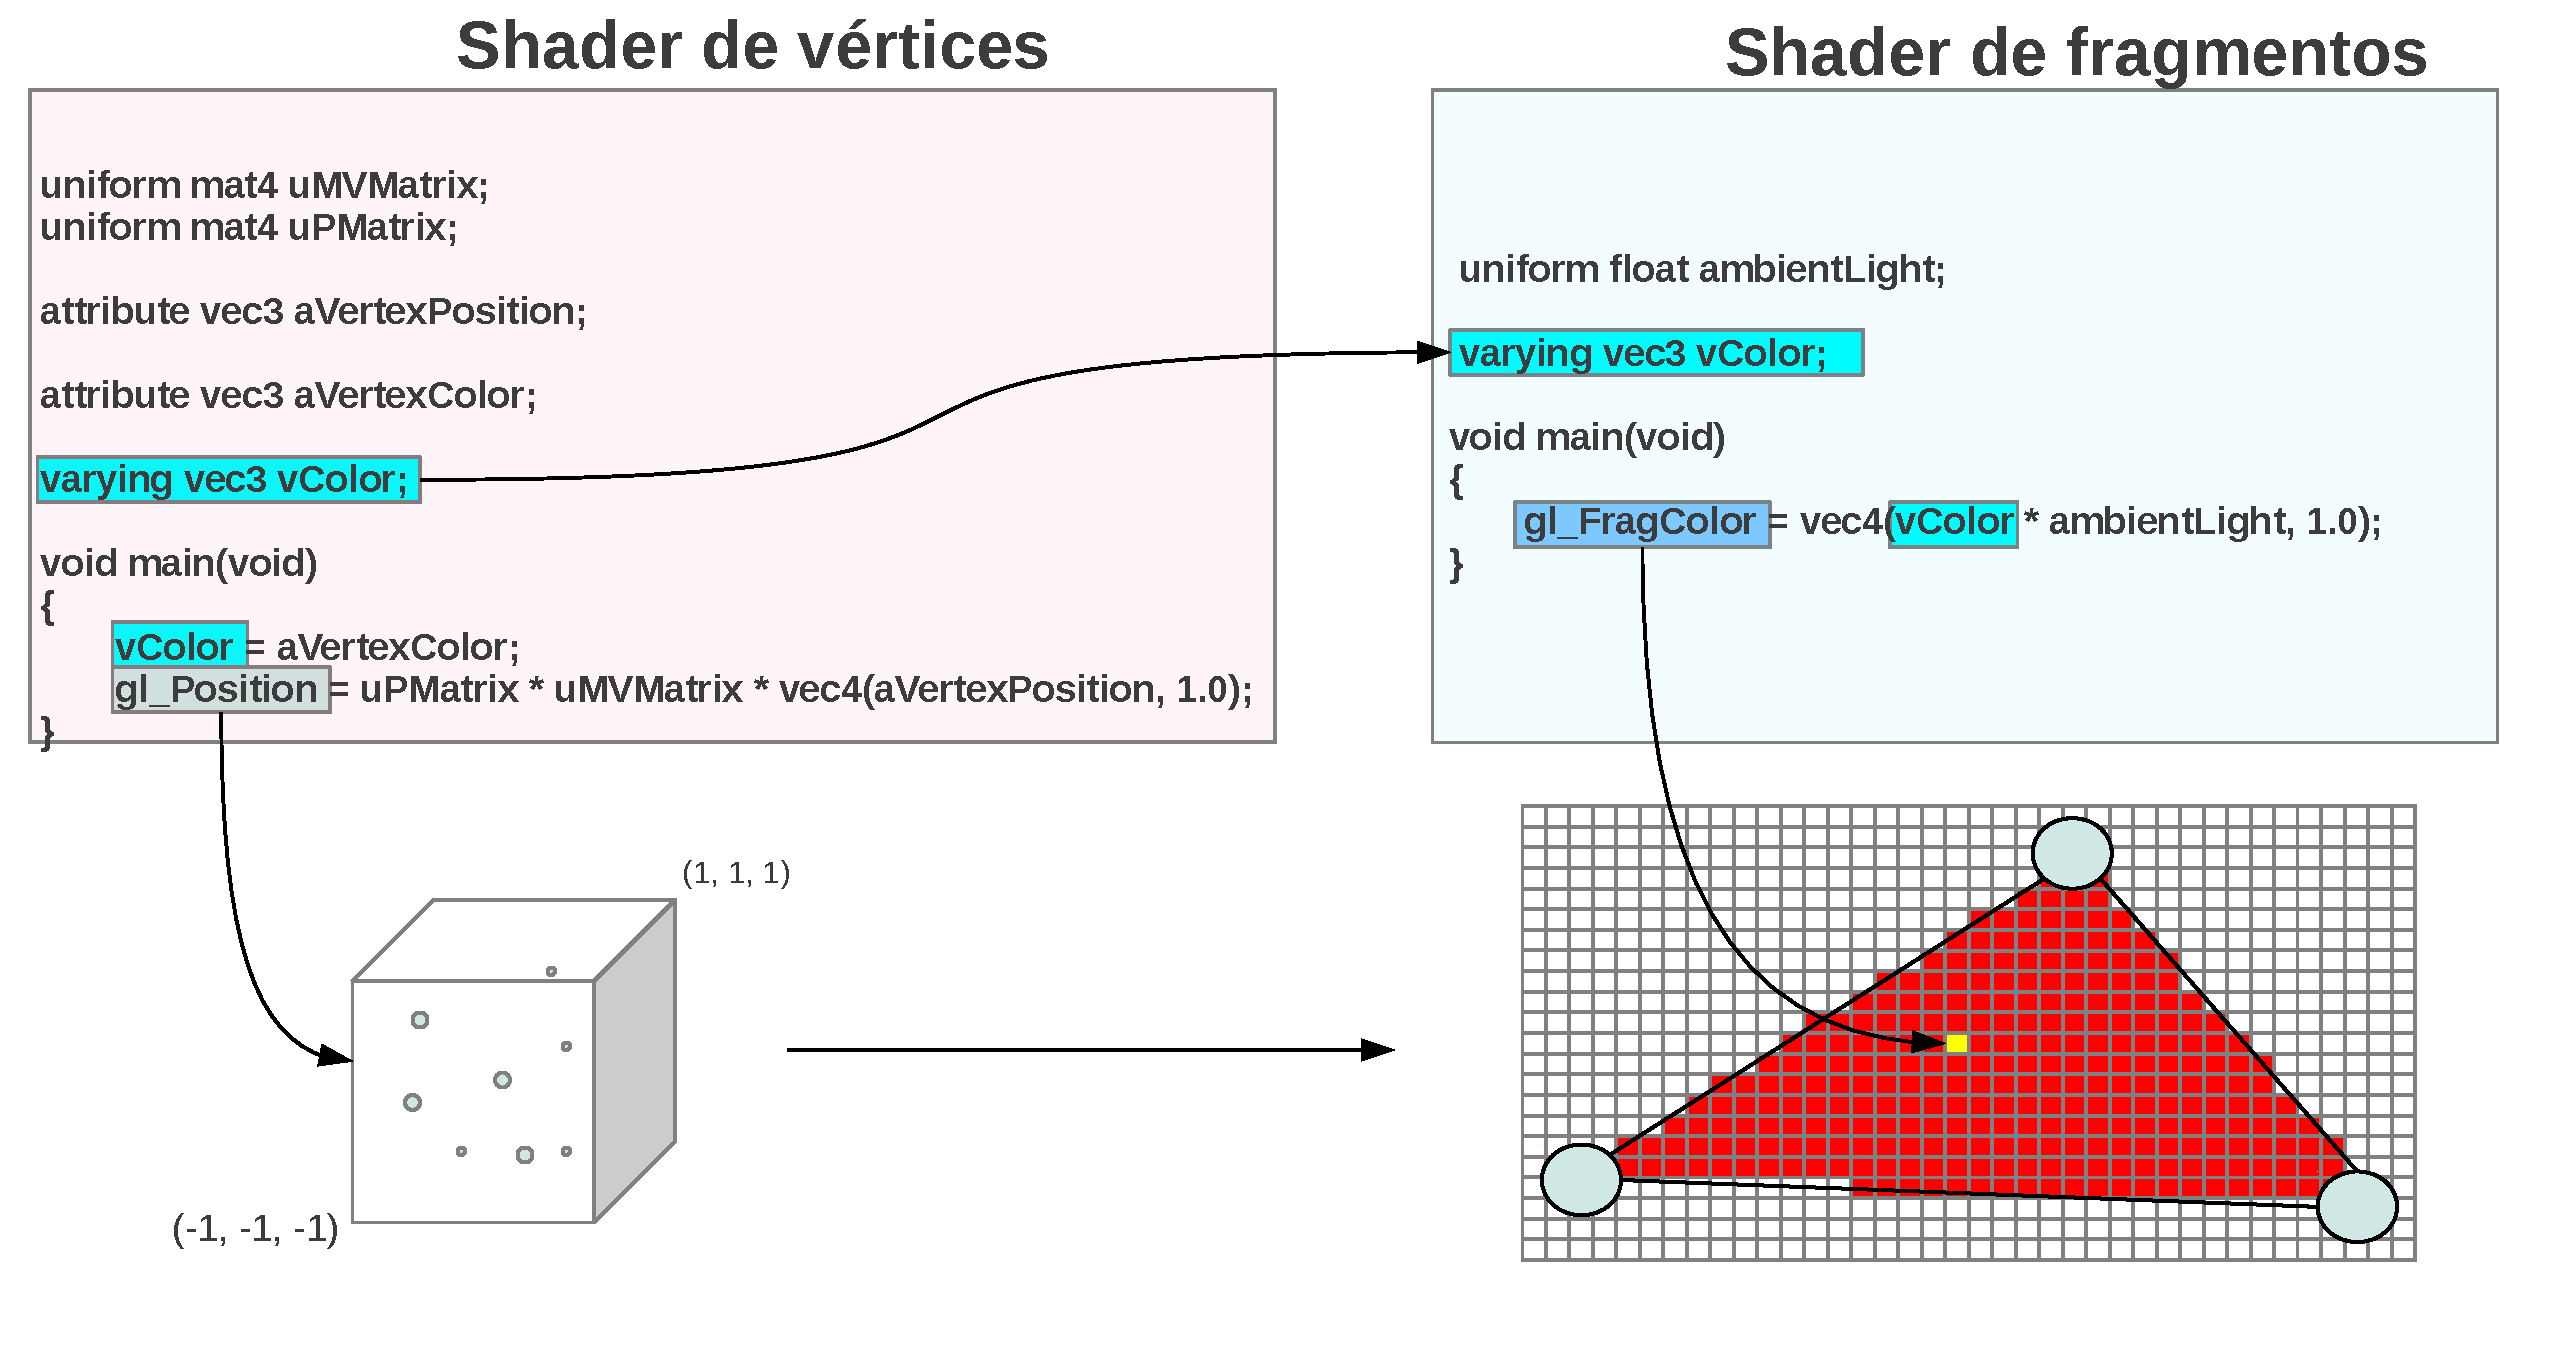
\includegraphics[width=13cm]{figures/fragmentshader}
\end{center}
\caption{Ejemplo de paso de datos del shader de vértices al shader de fragmentos.}
\label{fg:fragmentshader}
\end{figure}

La Fig.~\ref{fg:interpolation} muestra el resultado de esta operación.

\begin{figure}[h]
\begin{center}
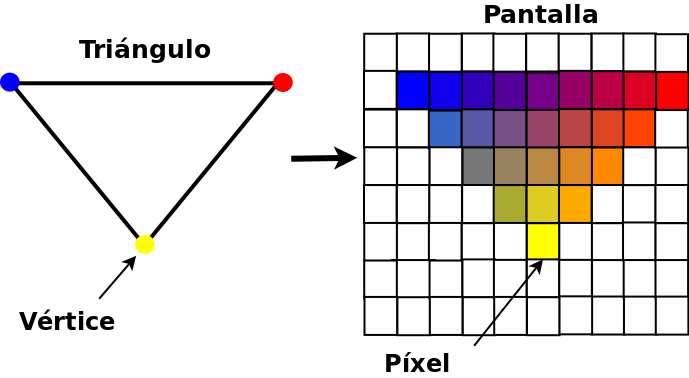
\includegraphics[width=8cm]{figures/interpolation}
\end{center}
\caption{Interpolación automática de colores en la GPU.}
\label{fg:interpolation}
\end{figure}



%Aquella informaci\'on que reciba como entrada debe presentar una {\em sem\'antica} asociada.
%Las {\em sem\'anticas} hacen que un elemento del programa cobre una significaci\'on especial, como puede ser la posici\'on, el color o una coordenada de una textura.
%Un ejemplo de código GLSL definiento un atributo es: 
%\begin{verbatim}
%attribute vec3 aVertexPosition;
%\end{verbatim}
%Indicando en este caso que la variable aVertexPosition hace referencia al atributo de posición en el espacio del vértice procesado.

%La sem\'antica es la palabra en may\'usculas que aparece despu\'es de los dos puntos. Aquella informaci\'on que devuelva el programa debe llevar la palabra clave {\em out}, la cual representa tambi\'en una sem\'antica. Es as\'i que {\em out} indica que ese elemento representa una salida del programa. He aqu\'i un ejemplo:

%\begin{verbatim}
%out float4 oPosition     : POSITION,
%\end{verbatim}

El Fragment Shader similarmente tiene par\'ametros de entrada y salida. Generalmente recibe el color interpolado por la etapa previa, tambi\'en puede recibir informaci\'on sobre texturas, codificada como coordenadas en las mismas. 

%Aqu\'i se presenta un ejemplo de las sem\'anticas:

%\begin{verbatim}
%float4 color 	 : COLOR
%float2 texCoord  : TEXCOORD0
%\end{verbatim}

%Indicando que las variables {\em color} y {\em texCoord} son par\'ametros de entrada. El cero al final del nombre de la segunda sem\'antica indica que nos referimos al primer par de coordenadas que se pueden recibir. Existen varios m\'as, dependiendo del perfil para el que se compile. 

Este shader a diferencia del primero, luego de realizar el procesamiento, s\'olo puede devolver un elemento, el {\em color} (excepto por algunos perfiles avanzados). Esta salida representa el color que, de pasar los diversos tests, tomar\'a el p\'ixel en pantalla.

Como fue dicho, existe otro tipo de objetos de entrada, los cuales llevan la palabra {\em uniform}. Los mismos representan objetos que son recibidos por el shader desde la aplicaci\'on.
%El principal atractivo de este tipo de objetos es hacer interactivos a los shaders, es decir, que desde la aplicaci\'on el usuario puede configurar valores que ser\'an utilizados en los shaders.

%\subsubsection{Tipos de Datos}
%Presentes en Cg est\'an los tipos de datos conocidos: {\em int}, {\em float}, y otros menos conocidos como {\em half} (punto flotante de menor precisi\'on, el cual es usado por eficiencia, puesto que requiere menor cantidad de recursos), as\'i como {\em arreglos}.

Al tener un enfoque gr\'afico, el lenguaje presenta tipos de datos de primer orden diferentes de lenguajes como C. Ejemplo de esto son los {\em vectores} y las {\em matrices}. Como se ha visto, GLSL tiene palabras reservadas para estos tipos de datos.
\begin{verbatim}
float f;
int a[4];
float2 v;
mat4 m;
\end{verbatim}
Aqu\'i se definen un flotante (f), un array de cuatro elementos enteros (a), un vector con dos componentes flotantes (v) y una matriz de 16 elementos de tipo flotante (m).
La diferencia entre un arreglo y un vector generalmente responde a la eficiencia.

Otros tipos de datos son los llamados {\em samplers}. Estos representan objetos externos a GLSL, como por ejemplo una textura.
Existen distintos tipos de samplers: {\em sampler1D}, {\em sampler2D} y {\em sampler3D}, representando respectivamente, objetos de una, dos y tres dimensiones. Tambi\'en tipos especiales como {\em samplerCUBE} (utilizado para t\'ecnicas como {\em environment mapping}) y {\em samplerRECT} (no posee dimensiones que son potencias de dos).

%Un ejemplo de uso es el siguiente:

%\begin{verbatim}
%function f(	float2 texCoord : TEXCOORD0, uniform sampler2D decal)
%{
%    tex2D(decal, texCoord);
%}
%\end{verbatim}

%La rutina tex2D consulta el objeto decal, en las coordenadas especificadas en texCoord, las cuales llegan como par\'ametro al programa. Este constituye un ejemplo t\'ipico de {\em texture mapping}.

\subsection{M\'as sobre el lenguaje}
Existe una biblioteca est\'andar que contiene funciones muy \'utiles para el programador. As\'i presenta funciones para realizar c\'alculos usuales como m\'aximos, m\'inimos, redondeos, seno, coseno, valores absolutos; y se le suman funciones para el trabajo con vectores, matrices y texturas, como {\em producto escalar}, {\em producto vectorial}, multiplicaci\'on de matrices, multiplicaci\'on de matriz y vector (y viceversa), obtenci\'on del valor de {\em texels} (como se ha visto).

En cuanto al lenguaje en s\'i, se utilizan {\em funciones} de la manera usual y con sintaxis similar a C.
Tambi\'en posee una funci\'on {\em principal} que se comporta como {\em main} en C.
La misma se especifica en la aplicaci\'on gr\'afica al crear una instancia de un programa GLSL, la cual entonces representa el punto de entrada al programa.
Tambi\'en se tienen estructuras de control usuales, como bucles {\em for} y {\em while}, aunque con determinadas restricciones dependiendo del perfil.

Se presenta a continuaci\'on otro tipo de lenguaje de programaci\'on, el cual permite realizar c\'alculo de prop\'osito general (GPGPU) en la GPU, a diferencia de los lenguajes de shader, que est\'a dise\~nado para utilizarse \'unicamente con fines gr\'aficos.

\section{GPGPU: CUDA y OpenCL}

\subsection{Introducci\'on}
La capacidad de procesamiento de las placas gr\'aficas ha ido evolucionado de manera vertiginosa hasta llegar al punto no s\'olo de rivalizar sino de superar en gran medida a los procesadores que se utilizan hoy en d\'ia.
Las mismas disponen de un n\'umero de {\em procesadores} en aumento por lo cual aparecen como dispositivos de procesamiento paralelo masivo.
Adem\'as, la velocidad de transmisi\'on de datos en su propia memoria tambi\'en es mucho mayor a la de un CPU tradicional.
Esto ocurre porque la CPU debe dedicar parte de su poder a control de flujo y {\em caching} de datos, en contraposici\'on la GPU est\'a dise\~nada para resolver problemas con un alto contenido de paralelismo; se debe aplicar el mismo programa a cada dato por lo cual el control de flujo es menos necesario.
Por estas razones, no es descabellado comenzar a pensar en utilizar la misma ya no como un dispositivo orientado \'unicamente a procesamiento de gr\'aficos, sino uno de procesamiento general.


Una de las primeras librerías fue desarrollada por la empresa NVIDIA: CUDA (siglas en ingl\'es de Compute Unified Device Architecture), una arquitectura de computaci\'on paralela de prop\'osito general para placas NVIDIA.
Además, el Khronos Group realiza la primera especificación del estándar abierto OpenCL \cite{Stone2010}.
El mismo representa un intento de que la computación paralela de propósito general (GPGPU) sea abierta y pueda implementarse en cualquier procesador.

\subsection{Paradigma de Programación en OpenCL}
Deben tenerse en cuenta ciertas consideraciones al implementar soluciones en OpenCL y CUDA.
En primer lugar, asistimos a un paradigma diferente al usual, ya que el cómputo se realiza en paralelo, a diferencia del computo secuencial tradicional de la máquina de Von Neumann.
Esto implica diversos cambios en la forma de programar una solución a un problema dado.

En su versión más simple, un programa secuencial es {\em trivialmente} paralelizable, si el cómputo es independiente para cada unidad del programa a ejecutar en cada procesador.
De esta forma, sólo debe chequearse la coherencia de los datos, es decir, que si por ejemplo sumamos dos arreglos, los índices en los arreglos de entrada que se suman se corresponda al índice correcto en el arreglo de salida.
Para esto, las bibliotecas que aquí tratamos tienen mecanismos de identificación global como fue explicado.
Entre los algoritmos trivialmente paralelizables encontramos aquellos que utilizan shaders (cómputos sobre vértices y píxeles independientes), suma de vectores y matrices, etc.

Sin embargo, la programación paralela trae aparejados problemas que fueron resueltos con cómputos secuenciales hace tiempo, y parcialmente olvidados por la historia de la computación con el paso de los años.
Entre ellos encontramos a los problemas de concurrencia.
Cuando diferentes procesadores trabajan sobre la misma memoria, debe programarse coherentemente los pasos, de tal forma de que el resultado sea el esperado.
Los problemas por regiones críticas (elementos de memoria que pueden ser modificados por más de una línea de trabajo) se multiplican en la programación paralela debido al número de procesos intervinientes.

Además de estas consideraciones, se encuentran otras dificultades inesperadas, como por ejemplo la utilización de condicionales (if), ya que, al ejecutar distintas ramas de un if, es posible perder mucha eficiencia.
Esto se debe a las diferencias de velocidad entre los distintos kernels, los cuales deben terminar todos al mismo tiempo un cómputo para poder proseguir con el siguiente grupo.
Es por esto que muchas veces la programación debe ser modificada para atender este nuevo objetivo.

Otras limitaciones tienen su causa en el estado actual del hardware gráfico.
Por ejemplo, la recursión aún no se permite en OpenCL, debido al posible consumo de memoria y registros en los procesadores, los cuales aún son limitados.
Debido a la misma causa, otro problema lo constituye la imposibilidad de solicitar memoria de la placa en tiempo de ejecución.

Por todos estos factores, la programación paralela en placas gráficas es aún dificultosa.
La elección de programación en GPU debe atender a la necesidad de un marcado crecimiento en la velocidad de ejecución del algoritmo en cuestión, y debe ser tomada teniendo en consideración todo lo expuesto aquí.

\section{Comparación GPU-CPU}
El paradigma de programación introducido en este apéndice ha demostrado un crecimiento en poder de cómputo prácticamente exponencial.
La Fig.~\ref{fg:cpugpu} muestra curvas con las capacidades en número de operaciones flotantes por segundo de las CPU y las GPU.
Puede observarse que las GPUs se presentan como un atractivo hardware que debe ser tenido en cuenta para aplicaciones donde los tiempos de cómputo resulten críticos.
Actualmente es imposible pensar en determinadas aplicaciones de tiempo real sin una implementación en GPU, y es por eso que en nuestra tesis hemos hecho hincapíé en esta tecnología.
La implementación del modelo de iluminación está basada en shaders ya que el cómputo resultó trivialmente paralelizable, resultando en un algoritmo de tiempo real.

\begin{figure}[h]
\begin{center}
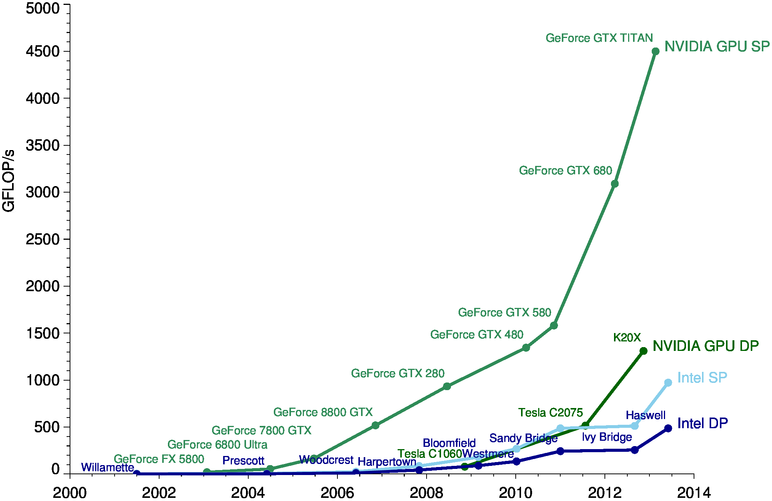
\includegraphics[width=12cm]{figures/cpugpu}
\end{center}
\caption[Comparación de velocidades de cómputo de la CPU y la GPU]{Comparación de velocidades de cómputo de la CPU y la GPU por medio del número de operaciones de punto flotante por segundo (FLOPS, fuente nVidia).}
\label{fg:cpugpu}
\end{figure}



\subsection{Entorno de programación CUDA}
En esta metodolog\'ia de programaci\'on, existen m\'ultiples hilos (threads) ejecutando en paralelo, ver Fig.~\ref{fg:cuda}.
Los threads son l\'ogicamente agrupados en {\em bloques} y son enumerados con un \'indice, as\'i hablamos del hilo $i$ de un determinado bloque (también es posible que estén organizados en más de una dimensión).
Los threads dentro de un bloque se ejecutan en el mismo procesador.
La cantidad de threads en un bloque queda limitada por los recursos de memoria del procesador de la GPU. Los bloques presentan la misma organizaci\'on, siendo categorizados en {\em grillas}. 
Por lo tanto se habla del bloque $j$ de una determinada grilla.
La memoria total de la GPU es llamada memoria global. Cada thread tiene su memoria local, s\'olo visible en ese thread.
A su vez, un block tiene su memoria local, la cual es compartida por todos los threads del mismo.
Por \'ultimo, todos los threads tienen acceso a la memoria {\em global} del grid.
Adem\'as, est\'an presentes la memoria de texturas y la memoria constante, las cuales son de s\'olo lectura.
Estas dos y la memoria global se preservan entre llamadas a {\em kernels} (ver siguiente secci\'on).

\begin{figure}[h]
\begin{center}
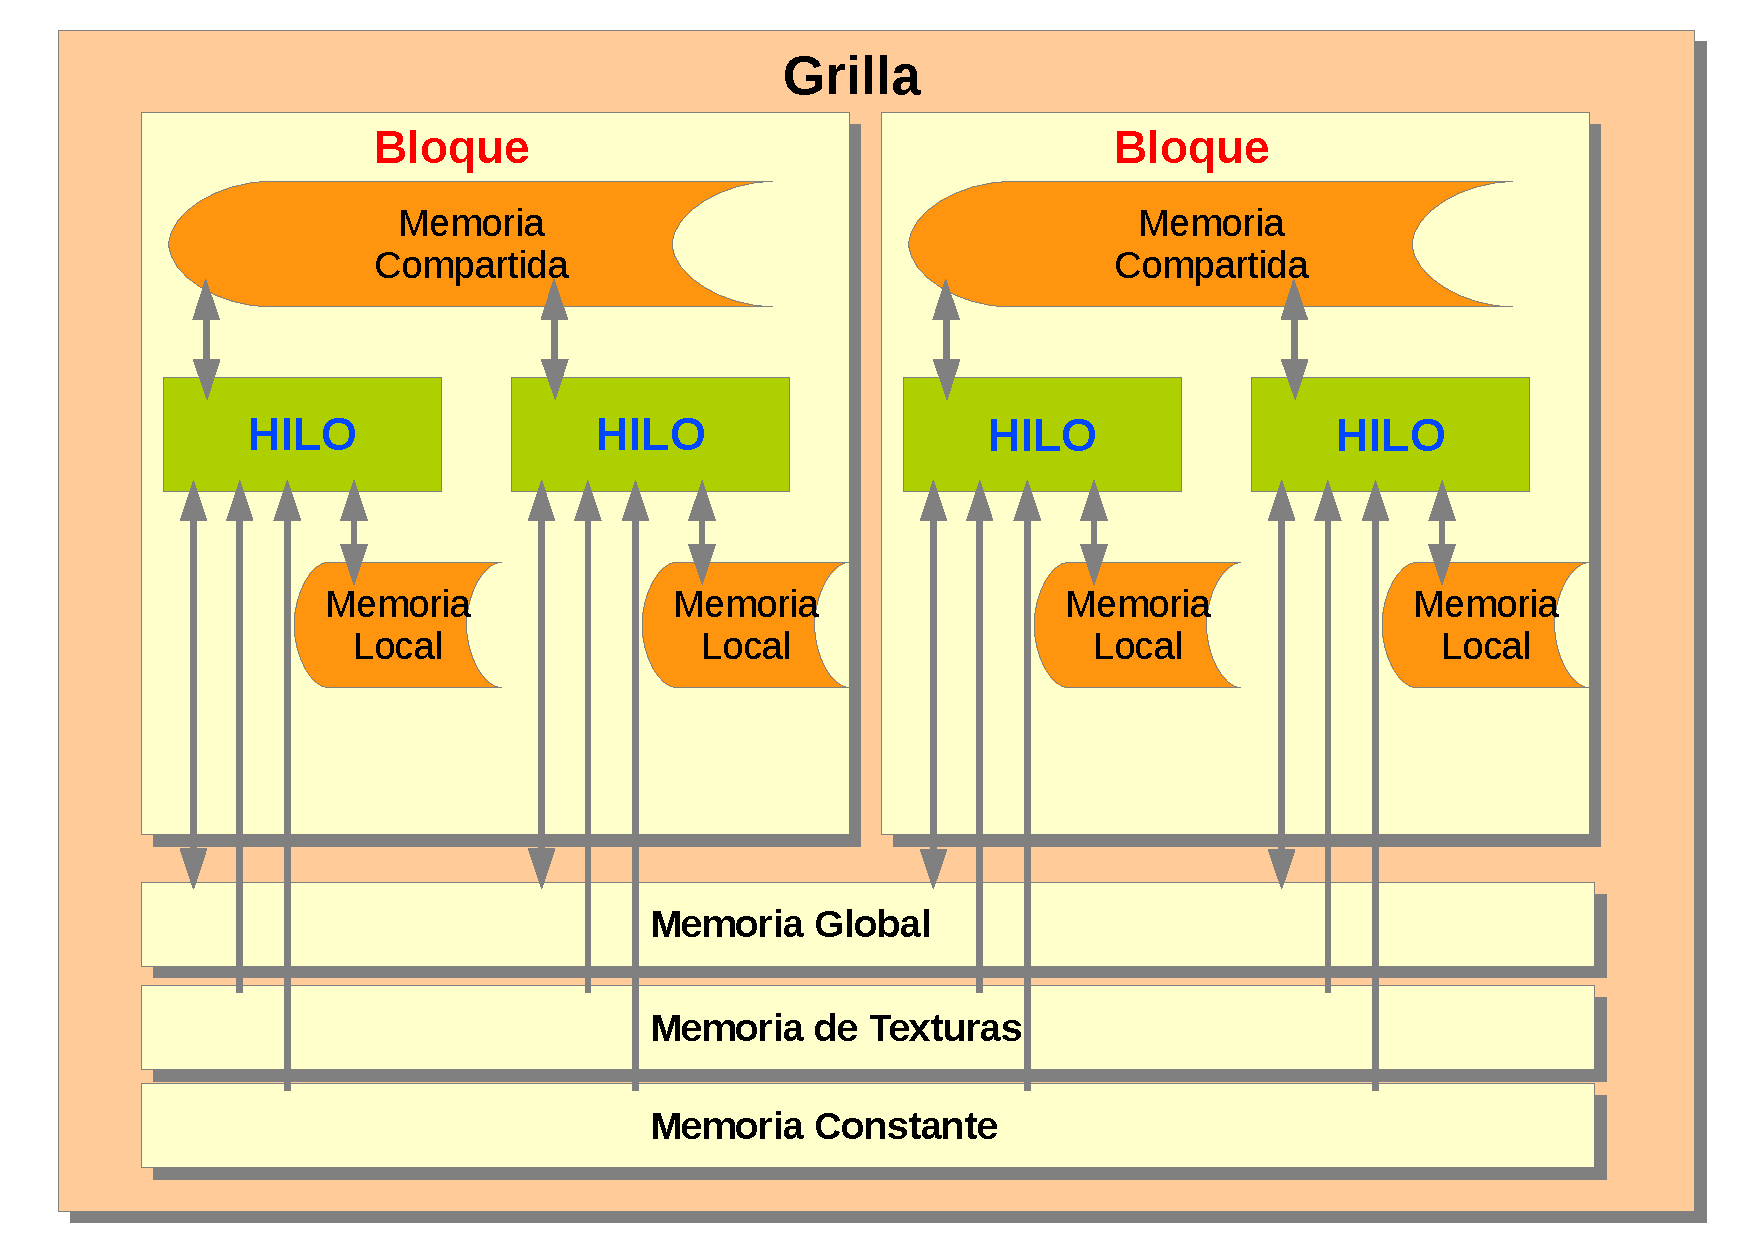
\includegraphics[width=13cm]{figures/cuda}
\end{center}
\caption{Arquitectura CUDA.}
\label{fg:cuda}
\end{figure}


\subsection{Programación en CUDA}
El software que provee CUDA permite a los programadores trabajar en un entorno C o Python (PyCUDA).
En un futuro otros lenguajes como {\em C++} y {\em FORTRAN} tambi\'en ser\'an soportados. 

Existen dos formas de escribir programas CUDA: {\em C para CUDA} y la {\em API del driver de CUDA}.
En el primer caso, se presenta como una extensi\'on a dicho lenguaje junto con un {\em runtime}.
El programador debe escribir funciones a ser ejecutadas en la GPU llamadas {\em kernels}. 
La principal diferencia con una funci\'on C convencional es que en lugar de ejecutarse secuencialmente, existen N threads paralelos ejecutando N instancias de dicha funci\'on. 
El creador del programa debe razonar el mismo como varios procesos a ejecutar en paralelo, los cuales unidos resuelven el problema.

He aqu\'i un ejemplo de un kernel, el cual suma dos vectores:

\begin{verbatim}
__global__ void VecAdd(float* A, float* B, float* C)
{
    int i = threadIdx.x;
    C[i] = A[i] + B[i];
}
\end{verbatim}

donde global se usa para definir el kernel y denota el car\'acter global del mismo.
La variable reservada threadIdx contiene el ID del thread dentro del block, que ejecuta la operaci\'on actual, la misma puede tener m\'as de una dimensi\'on, aunque en este caso tiene una sola y por lo tanto se accede al miembro x de la misma.
Para entender el kernel, debe comprenderse que cada thread sumar\'a un s\'olo elemento del vector final).
Ejecutar este kernel es tan sencillo como una llamada en C, con una salvedad: debe especificarse la cantidad de bloques por grilla (A) y la de hilos por bloque (B), bajo la sintaxis:
$$<<<A , B >>>$$

\begin{verbatim}
int main() {
    int N = 10;
    float* A;
    float* B;
    float* C;
    VecAdd<<<1, N>>>(A, B, C);
}

\end{verbatim}


El driver de CUDA es una API de un nivel de abstracci\'on m\'as bajo que el runtime.
De hecho, el runtime est\'a escrito sobre este API.
Su idea principal es cargar assembler o c\'odigo binario CUDA, y poder ejecutarlo.
Este c\'odigo se obtiene compilando un kernel.
En este modo tenemos m\'as control sobre lo que ocurre en la GPU, pero tambi\'en es m\'as dificultosa la programaci\'on y el {\em debug} del c\'odigo.
Ambos modos proveen m\'etodos para alocar memoria en la GPU, transferirla al CPU, manejar m\'ultiples GPU's, etc.
C para CUDA tiene la opci\'on de emular dispositivos f\'isicos en ausencia de ellos, lo cual puede resultar \'util en caso de no estar los mismos presentes.

\subsection{NVCC}
CUDA provee un compilador llamado {\em nvcc}.
El mismo se encarga de traducir nuestro c\'odigo hacia c\'odigo objeto.
Presenta una l\'inea de comandos similar a otros compiladores C como gcc, para facilitar su uso.
Normalmente, un fuente contiene c\'odigo del host y del device mezclado.
Por lo tanto, el esquema normal de trabajo del compilador consiste en separar c\'odigo a ejecutar en el host del c\'odigo a ejecutar en el device y traducir este \'ultimo hacia assembler ({\em PTX}) o c\'odigo objeto ({\em cubin}).
El c\'odigo del host encontrado en este proceso debe luego ser compilado con un compilador C o bien nvcc puede invocar al mismo y luego producir c\'odigo objeto directamente.

\subsection{cufft}
Esta biblioteca implementa algoritmos que permiten aplicar la transformada de Fourier directa e inversa a im\'agenes de una o m\'as dimensiones.
De este modo, podremos realizar la convoluci\'on de dos funciones aplicando s\'olo transformadas directas e inversas (por el teorema de convoluci\'on).
Como su nombre lo indica, la biblioteca utiliza el algoritmo {\em fft}, fast fourier transform, el cual aprovecha la propiedad de separabilidad de la transformada de fourier para computar la misma rápidamente.


\subsection{OpenCL}
Dada las similitudes entre CUDA y OpenCL, nos limitaremos aquí a exponer las principales diferencias entre ambas plataformas.

En primer lugar, debe tenerse en cuenta que si bien la creación de OpenCL está basada en la necesidad de explotación de una placa gráfica, en realidad el diseño de la especificación asume la computación en {\em cualquier} unidad con procesadores.
Es decir que OpenCL también puede correr en la CPU, por ejemplo.

Debido a esto, los nombres que fueron presentados previamente son más abstractos.
Cada procesador o placa gráfica que implementa el estándar es llamada dispositivo o device OpenCL. Cada dispositivo expone una cantidad de unidades de cómputo, o compute units. Estas unidades de cómputo son grupos de uno o más procesadores.
Los procesadores que forman parte de una unidad de cómputo son llamados elementos
de procesamiento o processing elements.
Todos los elementos de procesamiento dentro de una misma unidad de cómputo comparten recursos, como memoria y cache.
Esto significa que todos los elementos de procesamiento de una misma unidad de cómputo ejecutan las mismas instrucciones, aunque posiblemente leyendo y escribiendo a lugares diferentes de la memoria. En el caso de expresiones condicionales (if, else) simplemente se desactivan los elementos de procesamiento correspondientes durante la ejecución de la rama condicional que no deben ejecutar.

La memoria en OpenCL es organizada de igual manera que en CUDA, con tres niveles de jerarquía, cada uno con sus tiempos de acceso (global, compartida y privada, en orden descendiente de jerarquía).

El término {\em kernel} refiere al trozo de código a ser ejecutado por una unidad de procesamiento, el cual está escrito en un lenguaje parecido a {\em C}.

Cada kernel será ejecutado en un {\em elemento de procesamiento}.
Un conjunto de kernels es agrupado en un grupo de trabajo, el cual es ejecutado en una {\em unidad de cómputo}.
Dado que el código que se escribe es el mismo para todos los kernels, para poder diferenciar cual kernel es el actual, se utiliza las función reservada $get\_global\_id(0)$, la cual devuelve el kernel actual dentro de todos los kernels.
Existe un límite a la cantidad de kernels dentro de las unidades de trabajo, pero no a la cantidad de kernels total a ejecutarse.
En caso de que la cantidad total de kernels exceda la capacidad de la GPU, ésta dividirá el trabajo, comenzando a ejecutar algunos grupos de ellos (grupos de trabajo), y una vez terminado esto, ejecutará los siguientes grupos.


La estructura genérica de código python que utiliza OpenCL puede verse a continuación,
donde primero se define un contexto junto a una cola de ejecución, luego se define el programa a partir de un kernel, se lo ejecuta, y se copia el resultado a un arreglo en la CPU.

\begin{verbatim}
Import pyopencl as cl
ctx      = cl.create_some_context()
queue    = cl.CommandQueue(ctx)

# definición programa
prg      = cl.Program(ctx, <kernel_code>).build()

# ejecutar en GPU
prg.main(queue, (N,N), None, <buffers>, <args>) 

# copiar resultado a CPU
cl.enqueue_read_buffer(queue, dest_buf, buf).wait()
\end{verbatim}

donde $kernel\_code$ es un código arbitrario OpenCL.
Un ejemplo de código real OpenCL puede verse a continuación, donde se suman dos arreglos aleatorios $a\_{np}$ y $b\_{np}$. El resultado final es copiado al arreglo en CPU $res\_np$ y mostrado por pantalla en la última línea de código.
Los kernels que se ejecutan en la GPU, en paralelo, toman dos arreglos globales de entrada $a\_g$ y $b\_g$, y un arreglo global con el resultado $res\_g$.
Utilizando el identificador global $gid$, es posible diferenciar el kernel ejecutándose, y por lo tanto el identificador se utiliza como índice en el arreglo resultante, y en los arreglos de entrada, garantizando que a la misma posición en el arreglo de entrada le corresponde la de salida.
El orden exacto de ejecución corresponde a la GPU, y el programador no debe preocuparse.
Sólo debe tenerse en cuenta la consideración previa, es decir, garantizar la coherencia de los resultados.

\begin{verbatim}
import numpy as np
import pyopencl as cl

a_np = np.random.rand(50000).astype(np.float32)
b_np = np.random.rand(50000).astype(np.float32)

ctx = cl.create_some_context()
queue = cl.CommandQueue(ctx)

mf = cl.mem_flags
a_g = cl.Buffer(ctx, mf.READ_ONLY | mf.COPY_HOST_PTR, hostbuf=a_np)
b_g = cl.Buffer(ctx, mf.READ_ONLY | mf.COPY_HOST_PTR, hostbuf=b_np)

prg = cl.Program(ctx, """
__kernel void sum(__global const float *a_g,
                  __global const float *b_g,
                  __global float *res_g) {
  int gid = get_global_id(0);
  res_g[gid] = a_g[gid] + b_g[gid];
}
""").build()

res_g = cl.Buffer(ctx, mf.WRITE_ONLY, a_np.nbytes)
prg.sum(queue, a_np.shape, None, a_g, b_g, res_g)

res_np = np.empty_like(a_np)
cl.enqueue_copy(queue, res_np, res_g)

# imprimir resultados
print res_np
\end{verbatim}

El identificador $get\_global\_id$ toma un parámetro que indica la cantidad de dimensiones en los que están agrupados los kernels.
Por ejemplo, si trabajáramos con matrices en lugar de arreglos, y decidiéramos multiplicarlas o sumarlas, los identificadores de los kernels podrían estar definidos de a pares.
De esta forma con el par $(get\_global\_id(0), get\_global\_id(1))$, podríamos identificar la fila y columna a la que corresponde el kernel actual, y diseñar nuestro algoritmo para que trabaje solamente sobre un elemento de la matriz actual.

%\section{Aceleración de Algoritmos Fractales en GPU}

%Citar trabajo scipyconar 2014
%\section{Fractales y Multifractales en Computación Gráfica}
\section{Aplicaciones}
Como fue demostrado, además de su utilización en la producción de películas, video juegos, y otras áreas relacionadas a la computación gráfica, la programación de placas gráficas se ha abierto recientemente al cómputo general, por lo que otras ramas de la ciencia han comenzado a utilizar el inmenso poder computacional que proveen.
Este es el caso de física, finanzas, procesamiento de audio y video, astronomía y determinadas ramas de la computación (por ejemplo aprendizaje automatizado, o big data), donde complejas simulaciones tienen lugar en tiempos más acotados gracias a esta nueva herramienta.

En la presente tesis, el poder de la placa gráfica se ha utilizado sobre todo en el cómputo de la aproximación de la ecuación RTE, obteniendo tasas de refresco en tiempo real.
No sólo su utilización fue de gran ayuda, sino que es indispensable para cualquier algoritmo gráfico moderno el poder ejecutarse en las mismas si se pretenden alcanzar tiempos interactivos.
